\documentclass[12pt]{article}
\usepackage[a4paper,margin=0.8in]{geometry} % 明確設定四邊
\usepackage{fontspec}
\usepackage{xeCJK}
\usepackage{titling} % 預設標題下移0.6in
\usepackage{amsmath} % 數學方程式
\usepackage{graphicx} %圖片
\usepackage{float} % 在導言區,讓圖片強制插在原地
\usepackage{xcolor} %字體加入顏色
\usepackage{hyperref} % 引入網址
\usepackage{physics} % 物理符號
\usepackage{wrapfig} % 文字環繞圖
\usepackage{array} % 表格對齊控制
\usepackage{caption}

\captionsetup{
    labelfont={footnotesize,bf},    % 標籤:小字體+粗體
   % 文字:小字體
}
% 手動定義中文數字(不含標點符號)
\newcommand{\chinese}[1]{%
  \ifcase#1 零\or 一\or 二\or 三\or 四\or 五\or 六\or 七\or 八\or 九\or 十\or
  十一\or 十二\or 十三\or 十四\or 十五\or 十六\or 十七\or 十八\or 十九\or 二十\fi
}

% 重新定義章節編號格式
\renewcommand{\thesection}{\chinese{\value{section}}}
\renewcommand{\thesubsection}{\chinese{\value{section}}、\arabic{subsection}}
\renewcommand{\theequation}{\chinese{\value{section}}.\arabic{equation}}
\renewcommand{\thesubsubsection}{\chinese{\value{section}}、\arabic{subsection}.\arabic{subsubsection}}
\renewcommand{\thefigure}{\chinese{\value{section}}.\arabic{figure}\ }

% 讓方程式計數器在每個section重置
\counterwithin{equation}{section}
\setmainfont{Times New Roman}
\setCJKmainfont{Kaiti TC}

\setlength{\droptitle}{-1in} % 上移標題1in
\title{2.assignment\_2.6.tex}
\author{空間二階精度MINMOD離散格式}
\setcounter{section}{0}

\begin{document}
\maketitle
\section{二維穩態擴散對流方程的一般離散型式}
\noindent 若
\[
\begin{array}{l}
    \text{(1)A流場被定義為V不可壓縮流場}\\[1.5ex]
    \text{(2)A流場被定義為GF穩態流動相應之流場}\\[1.5ex]
    \text{(3)不考慮A流場的黏性應力耗散項$\Phi$}\\[1.5ex]
\end{array}
\]
則:
\begin{equation}\begin{split}
    &\text{A流場的能量方程式被定義為:}\\[1.5ex]
    &\vec{u}\cdot \vec{\nabla}T = -\vec{\nabla} \cdot (\Gamma \vec{\nabla}T) \\[1.5ex]
\end{split}\end{equation}
\noindent 上式$\vec{u}\cdot \vec{\nabla}T = -\vec{\nabla} \cdot (\Gamma \vec{\nabla}T)$
即被稱為穩態擴散對流方程的微分形式。若對上式取體積分,並引入連續方程式,則有:
\begin{equation}\begin{split}
    \oint_{\partial \Omega} \vec{da}\cdot (\vec{u}T) = \oint_{\partial \Omega} \vec{da}\cdot (\Gamma \vec{\nabla }T)
\end{split}\end{equation}
\noindent 上式即稱為穩態擴散對流方程的積分形式。若取(W((D二維穩態擴散對流方程)的(積分形式))的(一般離散格式)),則有:
\begin{equation}\begin{split}
    &A_{e}u_{e}T_{e} - A_{w}u_{w}T_{w}+A_{n}u_{n}T_{n} - A_{s}u_{s}T_{s} \\[1.5ex]
    =& A_{e}\Gamma_{e}\left.\frac{\partial T}{\partial x}\right|_{e}-A_{w}\Gamma_{w}\left.\frac{\partial T}{\partial x}\right|_{w}+A_{n}\Gamma_{n}\left.\frac{\partial T}{\partial y}\right|_{n}-A_{s}\Gamma_{s}\left.\frac{\partial T}{\partial y}\right|_{s}
\end{split}\end{equation}
\noindent 其中,各變量的下標$w,e,s,n$分別代表該變量在點$(i+\frac{1}{2},j),(i-\frac{1}{2},j),(i,j+\frac{1}{2}),(i,j-\frac{1}{2})$取值。
\noindent 進一步的,在一般離散格式中,對各邊界中心點的溫度場的一階法向導數取二階精度中心差分:
\begin{equation*}\begin{split}
    &\text{(U(E(S溫度場)的(一階法向偏導數))的(二階精度中心差分))}\\[1.5ex]
    &\left.\frac{\partial T}{\partial x}\right|_{e} \approx \frac{T_{E}-T_{P}}{\delta x}, \quad \left.\frac{\partial T}{\partial x}\right|_{w} \approx \frac{T_{P}-T_{W}}{\delta x}\\[1.5ex]
    &\left.\frac{\partial T}{\partial y}\right|_{n} \approx \frac{T_{N}-T_{P}}{\delta y}, \quad \left.\frac{\partial T}{\partial y}\right|_{s} \approx \frac{T_{P}-T_{S}}{\delta y}\\[1.5ex]
\end{split}\end{equation*}
\noindent 因此有:(W((D二維穩態擴散對流方程)的(積分形式))的(一般離散格式)):
\begin{equation}\begin{split}
     &A_{e}u_{e}T_{e} - A_{w}u_{w}T_{w}+A_{n}u_{n}T_{n} - A_{s}u_{s}T_{s} \\[1.5ex]
    =& A_{e}\Gamma_{e}\frac{T_{E}-T_{P}}{\delta x}-A_{w}\Gamma_{w}\frac{T_{P}-T_{W}}{\delta x}+A_{n}\Gamma_{n}\frac{T_{N}-T_{P}}{\delta y}-A_{s}\Gamma_{s}\frac{T_{P}-T_{S}}{\delta y}
\end{split}\end{equation}
\noindent 在二維均勻正交網格中,$A_{e} =A_{w} = \delta y , A_{n} = A_{s} = \delta x$,且令熱擴散係數$\Gamma$為常數,上式亦有如下形式之簡化:
\begin{equation}\begin{split}
     &\delta y\cdot  u_{e}T_{e} - \delta y\cdot u_{w}T_{w}+\delta x\cdot u_{n}T_{n} - \delta x\cdot u_{s}T_{s} \\[1.5ex]
    =& \delta y\cdot \Gamma\frac{T_{E}-T_{P}}{\delta x}-\delta y\cdot \Gamma\frac{T_{P}-T_{W}}{\delta x}+\delta x\cdot \Gamma\frac{T_{N}-T_{P}}{\delta y}-\delta x\cdot \Gamma\frac{T_{P}-T_{S}}{\delta y}\\[1.5ex]
    =& \Gamma(-2\frac{\delta y}{\delta x}-2\frac{\delta x}{\delta y})T_{P} + \Gamma\frac{\delta y}{\delta x}T_{W} + \Gamma\frac{\delta y}{\delta x}T_{E} + \Gamma\frac{\delta x}{\delta y}T_{S} + \Gamma\frac{\delta x}{\delta y}T_{N} \\[1.5ex]
\end{split}\end{equation}
\noindent 若在二維均勻正方網格中,(ie.對於每一個網格而言,$A_{e} = A_{w} = \delta y = \delta x = A_{n} = A_{s}$),上式又可以做如下簡化:
\begin{equation}\label{eq:general}\begin{split}
    &\delta y\cdot u_{e}T_{e} - \delta y\cdot u_{w}T_{w}+\delta x\cdot u_{n}T_{n} - \delta x\cdot u_{s}T_{s} \\[1.5ex]
    =& -4\Gamma T_{P} + \Gamma T_{W} + \Gamma T_{E} + \Gamma  T_{S} + \Gamma T_{N} \\[1.5ex]
\end{split}\end{equation}
\section{MINMOD格式}
\subsection{MINMOD近似取值}
\noindent 在空間二階精度MINMOD格式中,(E(r(p計算點)的(邊界中心點))的(溫度場))有如下取值:
\begin{equation*}\begin{split}
    &T_{f} = D(r_{f})T_{D}+U(r_{f})T_{U}+UU(r_{f})T_{UU}\\[1.5ex]
    &\text{其中,}\\
    &D(r_{f}<0) = 0\quad,\quad D(0 \leq r_{f}<1) = 0 \quad,\quad D(1 \leq r_{f}) = \frac{1}{2}  \\[1.5ex]
    &U(r_{f}<0) = \frac{2}{2}\quad,\quad U(0 \leq r_{f}<1) = \frac{3}{2}\quad,\quad U(1 \leq r_{f}) = \frac{1}{2} \\[1.5ex]
    &UU(r_{f}<0) = 0\quad,\quad UU(0 \leq r_{f}<1) = \frac{-1}{2}\quad,\quad UU(1 \leq r_{f}) = 0 \\[1.5ex] 
\end{split}\end{equation*}
\noindent 其中,下標f代表計算點p的某一個邊界中心點,且$r_{f} = \frac{T_{U} - T_{UU}}{T_{D} - T_{U}}$
接下來,我們從式\ref{eq:general}出發,帶入上述(U(E(r(p計算點)的(邊界中心點))的(溫度場))的(空間二階精度MINMOD近似取值)),則有:
(令$(u_{w},u_{e},u_{s},u_{n}) = (1,1,1,1)$)
\begin{equation}\begin{split}
     &\delta y \cdot (D(r_{e})T_{E}+(U(r_{e})-D(r_{w}))T_{P}+(UU(r_{e})-U(r_{w}))T_{W} -UU(r_{w})T_{WW})\\[1.5ex]
    +&\delta x \cdot (D(r_{n})T_{N}+(U(r_{n})-D(r_{s}))T_{P}+(UU(r_{n})-U(r_{s}))T_{S} -UU(r_{s})T_{SS})\\[1.5ex]
    =& -4\Gamma T_{P} + \Gamma T_{W} + \Gamma T_{E} + \Gamma  T_{S} + \Gamma T_{N} \\[1.5ex]
\end{split}\end{equation}
\noindent 編程提醒:\\[1.5ex]
\noindent 在編輯程式的過程中,最好將$r_{f}$設為矩陣形式,跟溫度場做連結,一但溫度場的更新,$r_{f}$跟著一起更新:
\begin{figure}[H]
    \centering
    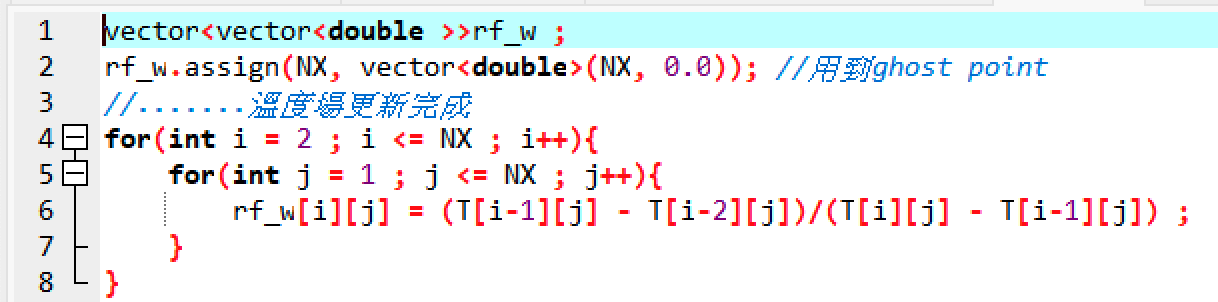
\includegraphics[width=0.6\textwidth]{29.png}
    \caption{$r_{f}$\footnotesize 更新示意圖}
    \label{fig:r_f更新}
\end{figure}
\subsection{內點的離散方程}
\noindent 定義域:i = [2,NX]$\quad,\quad$ j = [2,NY]\\[1.5ex]
\noindent 方程式:2D-steady advection-diffusion equation\\[1.5ex]
\noindent 方法:space second-order MINMOD scheme\\[1.5ex]
\noindent 對於每一個內點$(i,j)$,二維穩態擴散對流方程的空間二階精度MINMOD離散格式為:\\
\begin{equation}\begin{split}
    &T_{P}(4\Gamma+ \delta y\cdot(U(r_{e})-D(r_{w}))+\delta x\cdot (U(r_{n})-D(r_{s})))\\[1.5ex]
    =&T_{E}(\Gamma-\delta y \cdot D(r_{e}))\\[1.5ex]
    +&T_{W}(\Gamma-\delta y \cdot (UU(r_{e})-U(r_{w})))\\[1.5ex]
    +&T_{WW}(-\delta y\cdot (UU(r_{w})))\\[1.5ex]
    +&T_{N}(\Gamma-\delta x \cdot D(r_{n}))\\[1.5ex]
    +&T_{S}(\Gamma-\delta x \cdot (UU(r_{n})-U(r_{s})))\\[1.5ex]
    +&T_{SS}(-\delta x\cdot (UU(r_{s}))) \\[1.5ex]
\end{split}\end{equation}
\subsection{虛擬節點的設置}
\noindent 對於內點而言,在一維穩態擴散對流方程的空間二階精度MINMOD離散格中,會用到四個點。相應的,在二維穩態擴散對流方程的間二階精度MINMOD離散格式中,會用到八個點。如下圖所示:

\noindent
\begin{minipage}[t]{0.48\textwidth}
    \centering
    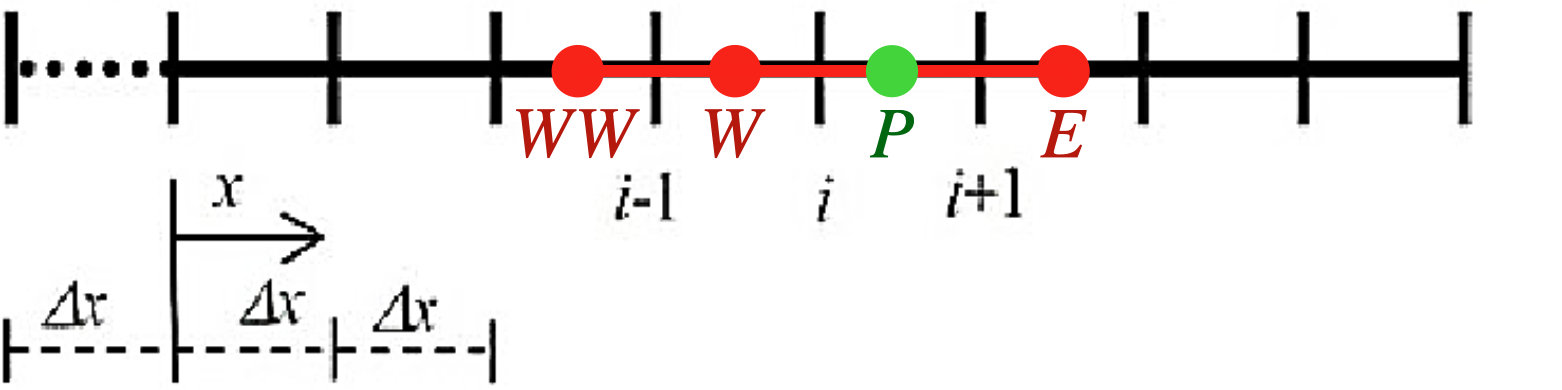
\includegraphics[width=0.8\textwidth]{31.png}
    \captionof{figure}{1D-4point stencil}
    \label{fig:1D-4point-stencil-1}
\end{minipage}
\hfill
\begin{minipage}[t]{0.48\textwidth}
    \centering
    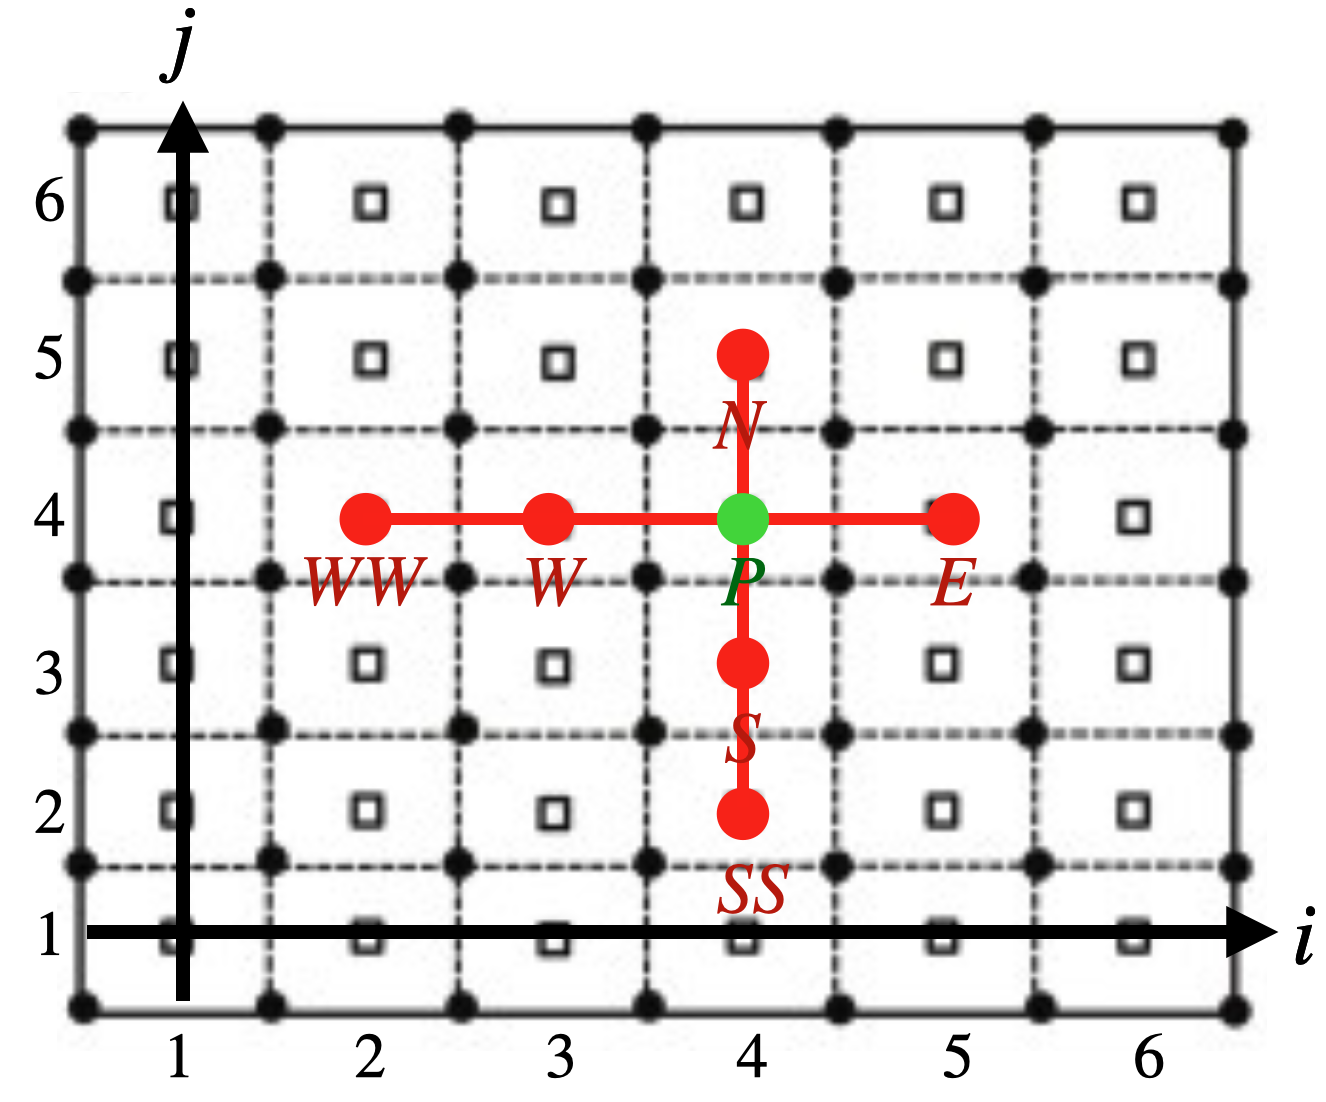
\includegraphics[width=0.8\textwidth]{30.png}
    \captionof{figure}{2D-8point stencil}
    \label{fig:2D-8point-stencil}
\end{minipage}\\[1.5ex]
\noindent 有三種情況會用到Ghost point (虛擬節點):
\subsubsection{MINMOD格式下的第一排邊界點}
\begin{figure}[H]
    \centering
    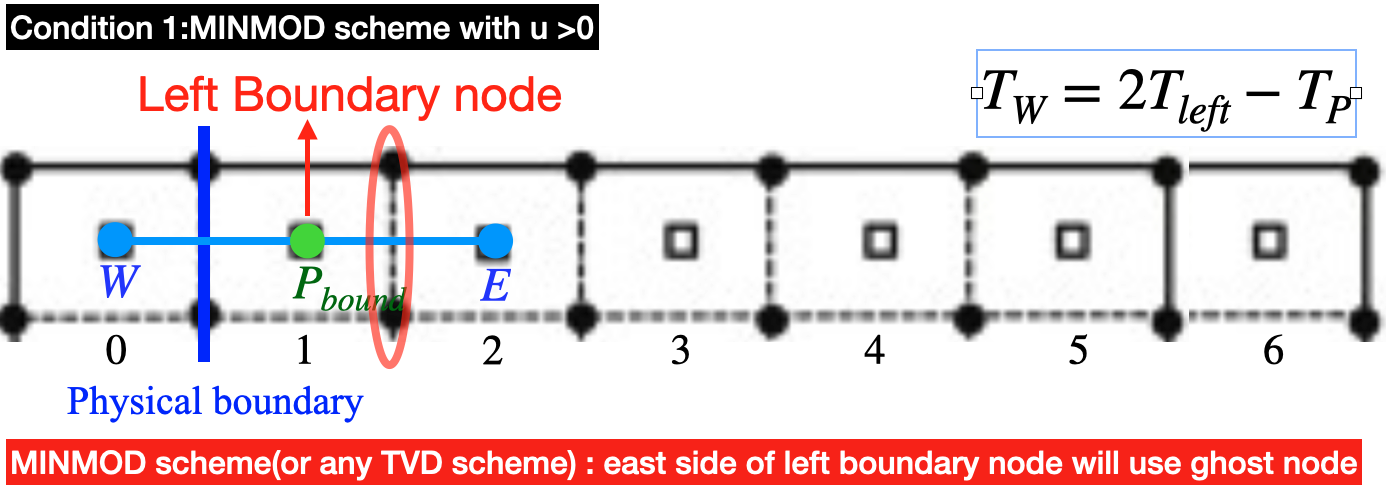
\includegraphics[width=0.6\textwidth]{33.png}
    \caption{\footnotesize MINMOD格式下的第一排邊界點}
    \label{fig:MINMOD格式下的第一排邊界點}
\end{figure}
\noindent 在迎風條件($u>0$)下,(Q(Y(E(p左邊界計算點)的(東邊界中心點))的(溫度場))的(空間二階精度MINMOD近似取值))會用到超出左邊界區域的計算點$W\ point\ ,\ T_{W}$,我們將其稱之為Ghost point (虛擬節點),並將其賦值為:$T_{W} = 2*T_{left} - T_{P}$。
\subsubsection{MINMOD格式下的第二排邊界點}
\begin{figure}[H]
    \centering
    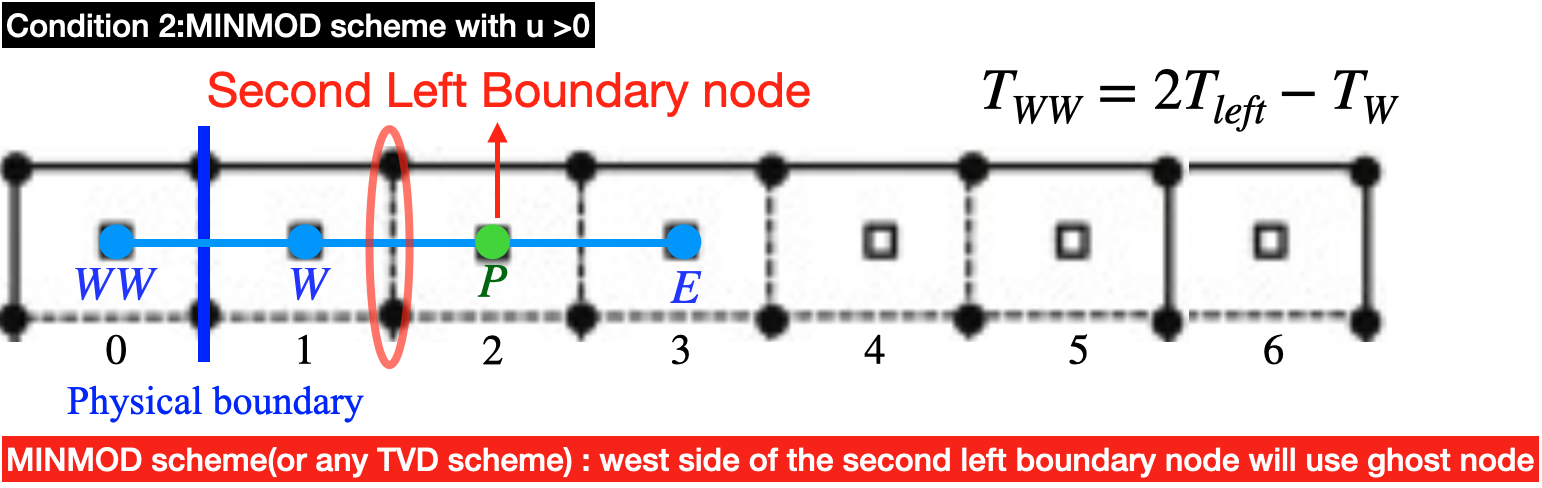
\includegraphics[width=0.6\textwidth]{34.png}
    \caption{\footnotesize MINMOD格式下的第二排邊界點}
    \label{fig:MINMOD格式下的第二排邊界點}
\end{figure}
\noindent 在迎風條件($u>0$)下,(H(L(E(i左邊界第二排計算點)的(西邊界中心點))的(溫度場))的(空間二階精度MINMOD近似取值))會用到超出左邊界區域的計算點$WW\ point\ ,\ T_{W}$,我們將其稱之為Ghost point (虛擬節點),並將其賦值為:$T_{H} = 2*T_{left} - T_{P}$。
\subsubsection{Neumann條件下的邊界點}
\begin{figure}[H]
    \centering
    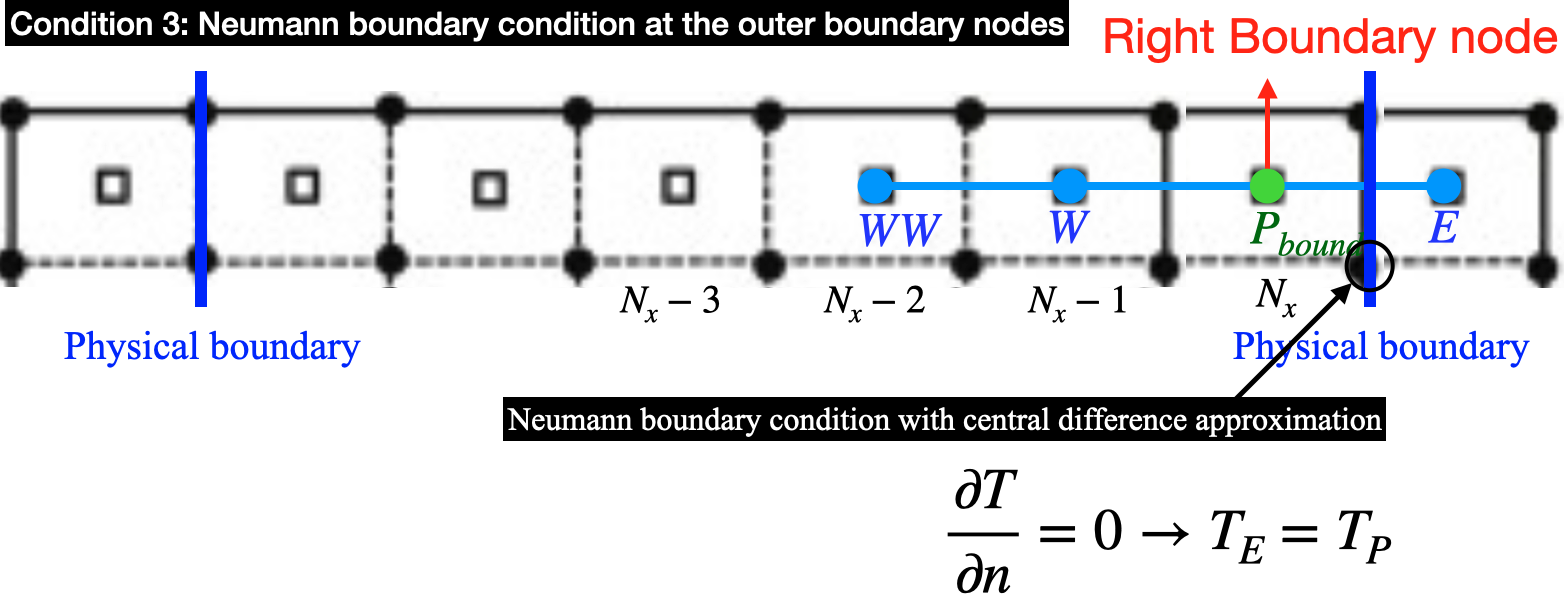
\includegraphics[width=0.6\textwidth]{35.png}
    \caption{\footnotesize Neumann條件下的邊界點}
    \label{fig:Neumann條件下的邊界點}
\end{figure}
\noindent Neumann條件為給定(E(D(T溫度場)的(一階法向偏導數))的(邊界函數)),呈如下函數式:$$\left. \frac{\partial T}{\partial n}\right|_{boundary} = g(\vec{r}) = 0$$ 
\noindent 此題中,所用到的Neumann條件為絕熱邊界條件,因此,在上邊界,有$\vec{n}\cdot \vec{\nabla }T = 0$而,在邊界上某一點(ex:$(i,N_{y})$),取(K(U(F(T溫度場)的(一階法向導數))的(邊界函數))的(二階精度中心差分)),有:
\begin{equation*}\begin{split}
    \left.\frac{\partial T}{\partial y}\right|_{i,N_{y}} \approx \frac{T_{i,N_{y}+1} - T_{i,N_{y}}}{\delta y}
\end{split}\end{equation*}
\noindent 因此,若(D(G(K(T溫度場)的(一階法向偏導數))的(邊界函數))的(二階精度中心差分)) = 0 恆成立,$$\frac{T_{i,N_{y}+1} - T_{i,N_{y}}}{\delta y} = 0$$,則(E(R(F(C上邊界計算點)的(北側邊界中心點))的(溫度場))的(近似取值))必然使用到Ghost point上的溫度場,且令Ghost point 上的溫度場為邊界計算點上未知待解的溫度場:$T_{P}$,因此,對於北邊界中心點的溫度場,可以近似取值為:\\[1.5ex]
\noindent (F(R(S(D上邊界計算點)的(北側邊界中心點))的(溫度場))的(空間二階精度MINMOD近似取值)):
\begin{equation}\begin{split}
    &for\ up\ boundary\ node (i,N_{y}):\\[1.5ex]
    &T_{n} = D(r_{n})T_{N} + U(r_{n})T_{P} + UU(r_{n})T_{S} \\[1.5ex]
    = &D(r_{n})T_{P} + U(r_{n})T_{P} + UU(r_{n})T_{S} \\[1.5ex]
\end{split}\end{equation}
\noindent (F(R(S(D上邊界計算點)的(北側邊界中心點))的(溫度場))的(空間二階精度UPWIND近似取值)):
\begin{equation}\begin{split}
    &for\ up\ boundary\ node (i,N_{y}):\\[1.5ex]
    &T_{n} = \frac{1}{2}T_{N} + \frac{3}{2}T_{P}  \\[1.5ex]
    =& \frac{1}{2}T_{P} + \frac{3}{2}T_{P}  \\[1.5ex]
\end{split}\end{equation}
\noindent 這些近似都可以很好的套用到邊界Neumann條件做使用。
\subsubsection{對流項的中心差分格式}
\begin{figure}[H]
    \centering
    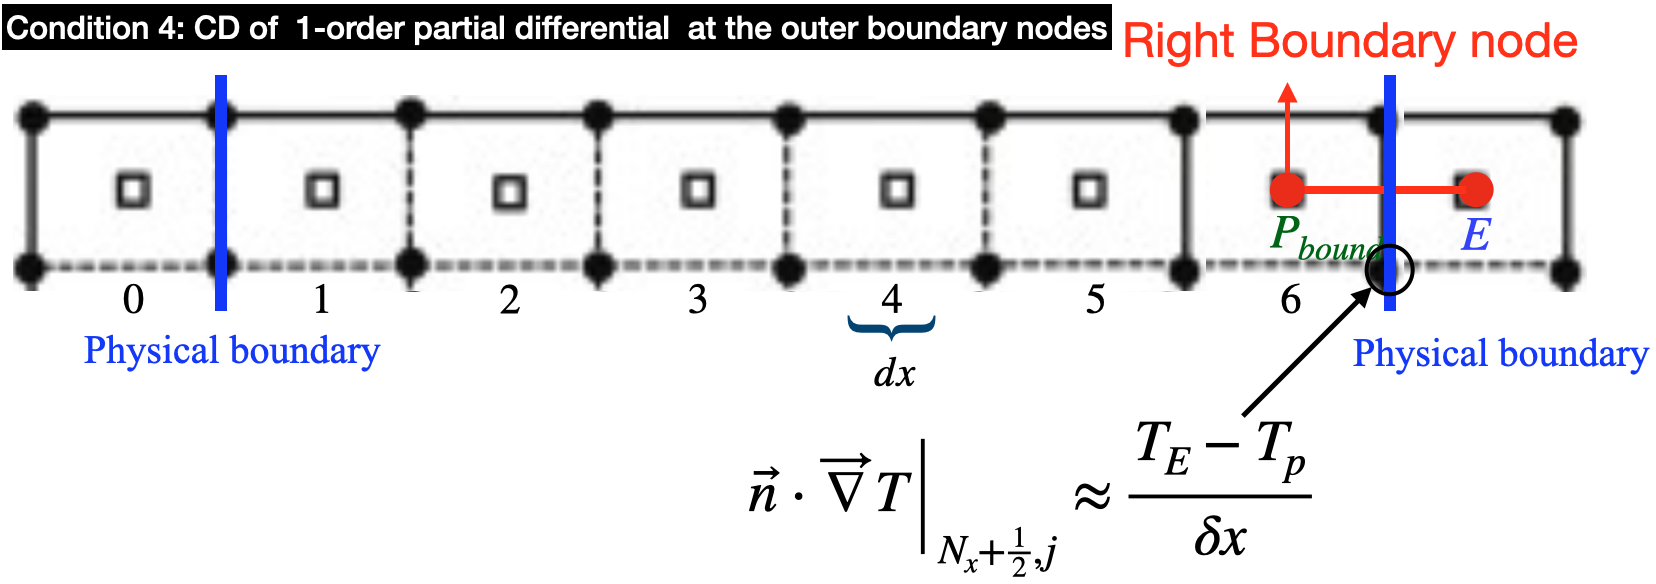
\includegraphics[width=0.6\textwidth]{37.png}
    \caption{\footnotesize 外側邊界上擴散項的二階精度中心差分}
    \label{fig:外側邊界上擴散項的二階精度中心差分}
\end{figure}
\noindent 對於邊界計算點而言,(E(S(T(F邊界計算點)的(外側邊界中心點))的(法向溫度梯度))的(二階精度中心差分)),會用到Ghost point上的溫度場,且令Ghost point 上的溫度場為$2T_{right} - T_{P}$。因此,外側邊界中心點的法向溫度梯度可以表示為:

\begin{equation}
    \left.\frac{\partial T}{\partial n}\right|_{e} \approx \frac{2(T_{right} - T_{P})}{\delta x}
\end{equation}
\subsubsection{二維虛擬節點的分佈}
\begin{figure}[H]
    \centering
    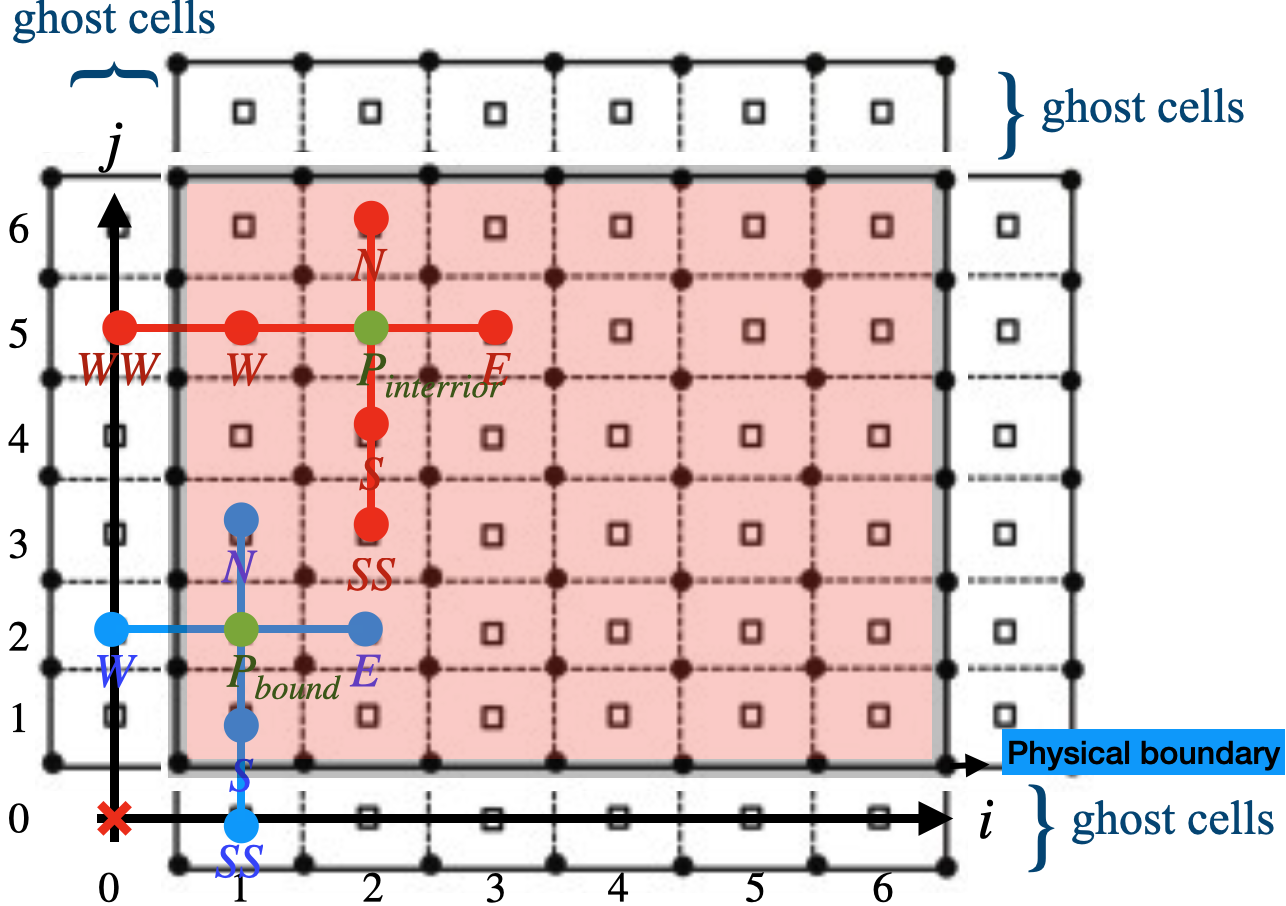
\includegraphics[width=0.6\textwidth]{32.png}
    \caption{\footnotesize 二維虛擬節點的分佈}
    \label{fig:二維虛擬節點的分佈}
\end{figure}
\noindent 在此二維問題中,\\
若\\[1.5ex]
(1)每一個計算點的邊界中心點的溫度場,近似取為(R(D(k(p計算點)的(邊界中心點))的(溫度場))的(空間二階精度MINMOD近似取值))\\[1.5ex]
(2)迎風條件:u>0 and v>0\\[1.5ex]
(3)Neumann條件:(D(G(K(T溫度場)的(一階法向偏導數))的(上邊界函數))的(二階精度中心差分)) = 0 恆成立\\[1.0ex]
則,對於全場計算點,((E二維穩態擴散對流方程)的(空間二階精度MINMOD離散格式))中,會用到的虛擬節點分佈如圖\ref{fig:二維虛擬節點的分佈}所示。
\subsection{邊界計算點的離散方程式}
\noindent 以下將討論各個邊界計算點上所滿足的離散方程。
\noindent 範圍:(包括四個邊界以及四格角點)
\[
\begin{array}{l}
    \text{(1)左邊界計算點($i = 1\ ,\ j \in [2,N_{y-1}]$)}\\[1.5ex]
    \text{(2)右邊界計算點($i = N_{x}\ ,\ j \in [2,N_{y-1}]$)}\\[1.5ex]
    \text{(3)下邊界計算點($i \in [2,N_{x}-1]\ ,\ j = 1$)}\\[1.5ex]
    \text{(4)上邊界計算點($i \in [2,N_{x}-1]\ ,\ j = N_{y}$)}\\[1.5ex]
\end{array}
\begin{array}{l}
    \text{(1)左下計算點($i = 1\ ,\ j = 1$)}\\[1.5ex]
    \text{(2)右下計算點($i = N_{x}\ ,\ j = 1$)}\\[1.5ex]
    \text{(3)左上計算點($i = 1\ ,\ j = N_{y}$)}\\[1.5ex]
    \text{(4)右上計算點($i = N_{x}\ ,\ j = N_{y}$)}\\[1.5ex]
\end{array}
\]
\noindent 格式:(S(R二維穩態擴散對流方程)的(空間二階精度MINMOD離散格式))\\[1.5ex]
注意:設置虛擬節點的範圍,以及虛擬節點上的溫度取值:
\[
\begin{array}{l}
    \text{(1)左邊界計算點之左延伸行計算點($i = 0\ ,\ j \in [2,N_{y-1}]$)}\\[1.5ex]
    \text{(2)右邊界計算點之右延伸行計算點($i = N_{x}+1\ ,\ j \in [2,N_{y-1}]$)}\\[1.5ex]
    \text{(3)下邊界計算點之下延伸列計算點($i \in [2,N_{x}-1]\ ,\ j = 0$)}\\[1.5ex]
    \text{(4)上邊界計算點之上延伸列計算點($i \in [2,N_{x}-1]\ ,\ j = N_{y}+1$)}\\[1.5ex]
\end{array}
\begin{array}{l}
    :\ T_{0,j} = 2*T_{left} - T_{1,j}\\[1.5ex]
    :\ T_{N_{x}+1,j} = 2*T_{right} - T_{N_{x},j}\\[1.5ex]
    :\ T_{i,0} = 2*T_{bottom} - T_{i,1}\\[1.5ex]
    :\ T_{i,N_{y}+1} = T_{i,N_{y}}\\[1.5ex]
\end{array}
\]
下圖為各個需要用到的ghost point 分布,以及該點ghost point 上的外差取值(用到邊界條件)。
\begin{figure}[H]
    \centering
    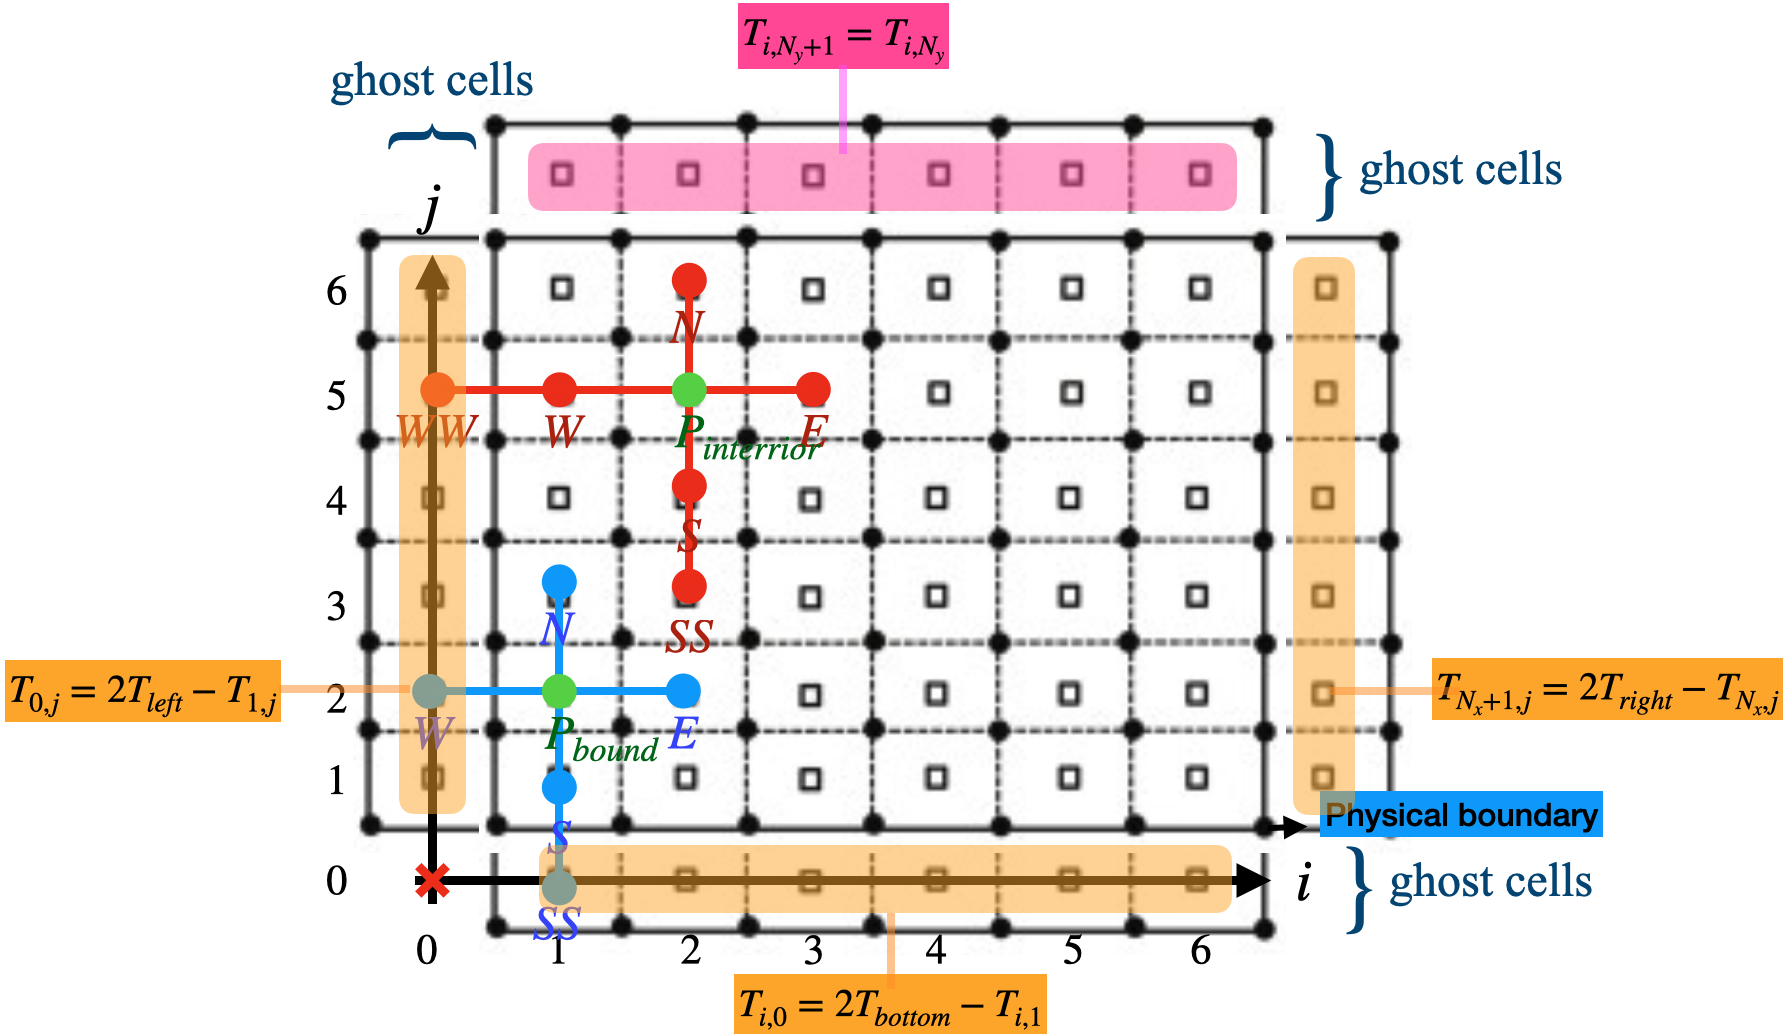
\includegraphics[width=0.6\textwidth]{38.png}
    \caption{\footnotesize ghost point predict value}
    \label{fig:ghost point predict value}
\end{figure}
\subsubsection{左邊界計算點}
\noindent 範圍:$i = 1\ ,\ j\in [2,N_{y}-1]$\\[1.5ex]
\noindent g左邊界計算點的(K(D二維穩態擴散對流方程)的(空間二階精度MINMOD離散格式))為:
\begin{equation}\begin{split}
&T_{P}(4\Gamma + \delta y(U(r_e)) + \delta x(U(r_n) - D(r_s)))\\[1.5ex]
=&T_{W}(\Gamma - \delta y(UU(r_e)))\\[1.5ex]
+&T_{E}(\Gamma - \delta y(D(r_e)) )\\[1.5ex]
+&T_{S}(\Gamma - \delta x(UU(r_n)-U(r_s)))\\[1.5ex]
+&T_{N}(\Gamma - \delta x(D(r_n)))\\[1.5ex]
+&T_{SS}(- \delta x(-UU(r_s)))\\[1.5ex]
+&T_{left}(+ \delta y)\\[1.5ex]
\end{split}\end{equation}
\subsubsection{右邊界計算點}
\noindent 範圍:$i = N_{x}\ ,\ j\in [2,N_{y}-1]$\\[1.5ex]
\noindent j右邊界計算點的(K'(D'二維穩態擴散對流方程)的(空間二階精度MINMOD離散格式))為:
\begin{equation}\begin{split}
&T_{P}(4\Gamma +\delta y(-D(r_w)) +\delta x(U(r_n)-D(r_s)))\\[1.5ex]
=&T_{W}(\Gamma -\delta y(-U(r_w)))\\[1.5ex]
+&T_{E}(\Gamma )\\[1.5ex]
+&T_{S}(\Gamma -\delta x(UU(r_n)-U(r_s)))\\[1.5ex]
+&T_{N}(\Gamma -\delta x(D(r_n)))\\[1.5ex]
\end{split}\end{equation}
\begin{equation}\begin{split}
+&T_{WW}(-\delta y(-UU(r_w)))\\[1.5ex]
+&T_{SS}(-\delta y(-UU(r_s)))\\[1.5ex]
-&T_{right}(\delta y)\\[1.5ex]
\end{split}\end{equation}
\subsubsection{下邊界計算點}
\noindent 範圍:$i \in [2,N_{x}-1]\ ,\ j = 1$\\[1.5ex]
\noindent p下邊界計算點的(K''(D''二維穩態擴散對流方程)的(空間二階精度MINMOD離散格式))為:
\begin{equation}\begin{split}
    &T_{P}(4\Gamma + \delta y (U(r_{e})- D(r_{w})) + \delta x (U(r_{n})))\\[1.5ex]
    =&T_{W}(\Gamma - \delta y (UU(r_{e}) - U(r_{w})))\\[1.5ex]
    +&T_{E}(\Gamma - \delta y (D(r_{e})))\\[1.5ex]
    +&T_{S}(\Gamma - \delta x (UU(r_{n})))\\[1.5ex]
    +&T_{N}(\Gamma - \delta x (D(r_{n})))\\[1.5ex]
    +&T_{WW}(-\delta y (-UU(r_{w})))\\[1.5ex] 
    +&dx\cdot T_{bottom}\\[1.5ex]
\end{split}\end{equation}
\subsubsection{上邊界計算點}
\noindent 範圍:$i \in [2,N_{x}-1]\ ,\ j = N_{y}$\\[1.5ex]
\noindent b上邊界計算點的(K'''(D'''二維穩態擴散對流方程)的(空間二精度MINMOD離散格式))為:
\begin{equation}\begin{split}
    &T_{P}(3\Gamma + \delta y (U(r_{e})-D(r_{w})) + \delta x (U(r_{n})-D(r_{s}))) \\[1.5ex]
    =&T_{W}(\Gamma - \delta y (UU(r_{e}) - U(r_{w})))\\[1.5ex]
    +&T_{E}(\Gamma - \delta y (D(r_{e})))\\[1.5ex]
    +&T_{S}(\Gamma - \delta x (UU(r_{n})-U(r_{s})))\\[1.5ex]
    +&T_{N}(- \delta x (D(r_{n})))\\[1.5ex]
    +&T_{WW}(-\delta y (-UU(r_{w})))\\[1.5ex]
    +&T_{SS}(- \delta x (-UU(r_{s})))\\[1.5ex]
\end{split}\end{equation}
上式為套用Neumann條件下的結果,基於Neumann條件,並沒有用到外源項。
\end{document}
